\documentclass[11pt]{scrartcl}

\usepackage[sexy]{evan}
\usepackage{import}
\usepackage[table]{xcolor}
\usepackage{xfp}
\usepackage{multicol}

\newcommand{\gad}{\textcolor{yellow}{$\bigstar$}}
\newcommand{\bad}{\textcolor{red}{$\bigstar$}}

\definecolor{dcol0}{HTML}{C8E6C9}
\definecolor{dcol1}{HTML}{D4E9B3}
\definecolor{dcol2}{HTML}{E5ED9A}
\definecolor{dcol3}{HTML}{FFF59D}
\definecolor{dcol4}{HTML}{FFE082}
\definecolor{dcol5}{HTML}{FFCC80}
\definecolor{dcol6}{HTML}{FFAB91}
\definecolor{dcol7}{HTML}{F49890}
\definecolor{dcol8}{HTML}{E57373}
\definecolor{dcol9}{HTML}{D32F2F}

\makeatletter
\newcommand{\getcolorname}[1]{dcol#1}
\makeatother

\newcommand{\dif}[1]{%
    \edef\colorindex{\number\fpeval{floor(#1)}}%
    \edef\fulltext{#1}%
    \colorbox{\getcolorname{\colorindex}}{%
        \ifnum\colorindex>8
            \textbf{\textcolor{white}{\,\fulltext\,}}%
        \else
            \textbf{\textcolor{black}{\,\fulltext\,}}%
        \fi
    }%
}
% Variable para dificultad (inicial 0)
\newcommand{\thmdifficulty}{0}

% Comando para asignar dificultad antes del problema
\newcommand{\problemdiff}[1]{\renewcommand{\thmdifficulty}{#1}}

% Estilo del problema que incluye dificultad antes del título
\declaretheoremstyle[
    headfont=\color{blue!40!black}\normalfont\bfseries,
    headformat={%
      \dif{\thmdifficulty}\quad \NAME~\NUMBER\ifx\relax\EMPTY\relax\else\ \NOTE\fi
    },
    postheadspace=1em,
    spaceabove=8pt,
    spacebelow=8pt,
    bodyfont=\normalfont
]{problemstyle}

    \declaretheorem[style=problemstyle,name=Problema,sibling=theorem]{problema}
    \declaretheorem[style=problemstyle,name=Problema,numbered=no]{problema*}

\definecolor{yellow4}{RGB}{255, 206, 0}

\title {GeoCombi}
\subtitle {Entrenamientos Nacionales Oros}

\author{Emmanuel Buenrostro}
\date{10 de Enero de 2026}

\begin{document}
\maketitle

\section{Teoría}

En esta parte voy a hablar sobre todo de distintas tecnicas útiles que sirven para atacar problemas de GeoCombi. Cabe aclarar que aunque no es mencionado aqui, la Inducción para obtener acomodos o para probar cosas también es bastante útil en GeoCombi. \\
\subsection{Casillas}
\begin{example}
    Prueba que entre cualesquiera 5 puntos en un triangulo equilatero de lado 1, hay 2 cuya distancia es máximo $\half$.
\end{example}

\begin{soln}
La prueba de esto es que si divides el triangulo en cuatro triangulos equilateros de lado $\half$ (esto trazando la union de los puntos medios de cada lado) entonces, por casillas, hay 2 puntos en el mismo triangulo y la distancia maxima en un triangulo equilatero de lado $\half$ es $\half$.
\end{soln}

\subsection{Principio Extremo}
\begin{example}
    Hay $2n$ puntos en el plano, de forma que no hay 3 colineales. $n$ son coloreados de azul y $n$ de rojo. Demuestra que puedes unir los $n$ puntos rojos a los $n$ puntos azules con $n$ segmentos (cada segmento une un punto rojo con uno azul), de forma que no hay dos segmentos que se intersecten. 
\end{example}

\begin{soln}
    Esta vez vamos a tomarnos un acomodo que minimice algo, en este caso vamos a minimizar la suma de los $n$ segmentos utilizados. \\
    Veamos que este acomodo funciona, ya que si dos segmentos $AB,CD$ se intersectan en $P$. Podemos ver que por desigualdad del triangulo: 

    \[AB+CD=AP+PB+CP+PD=(AP+PD)+(CP+PB) > AD+CB\]
    \begin{center}
        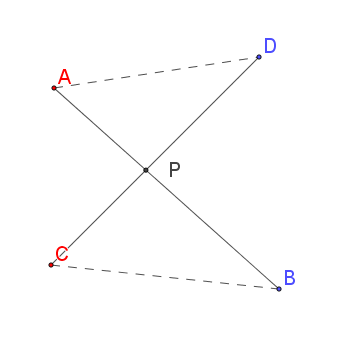
\includegraphics[scale=0.5]{IMG1.png}
    \end{center}
    Podrias tomar ese acomodo y haria que la suma sea menor, contradiciendo la minimicidad del acomodo, entonces ese acomodo si cumple las condiciones.

\end{soln}

\subsection{Barridos / Orientación de Ejes }

\begin{definition}
    [Posición general]
    Decimos que un conjunto de puntos esta en posición general si no hay 3 colineales. \\
    Decimos que un conjunto de rectas esta en posición general si no hay 3 rectas concurrentes, ni 2 rectas paralelas.
\end{definition}

\begin{example}
    [Regional Centro 2018/3]
    Considera $n$ rectas en el plano en posición general. Determina si es posible etiquetar los $k$ puntos de intersección de estas rectas del $1$ al $k$ (usando cada número exactamente una vez), de forma que en cada recta, las etiquetas de los $n-1$ puntos aparezcan en orden creciente (en alguna de las direcciones en las que se puede recorrer). 
\end{example}

\begin{soln}
    Al trabajar con planos y númeraciones, muchas veces ordenar los puntos en base a sus coordenadas $(x,y)$ es muy util, pero para definir esas coordenadas necesitamos definir sus ejes. \\
    Los ejes pueden ser cualquier pareja de rectas tales que sean perpendiculares. \\

        Entonces para este problema vamos a escoger un eje $y$ tal que ninguna recta sea paralela de nuestro conjunto sea paralela a el eje. (Existen infinitas posibles pendientes y en el conjunto usas una cantidad finita, entonces existe una pendiente que puede ser la recta del nuevo eje $y$.) \\
        Entonces ordenamos los puntos de intersección $(x,y)$ de forma que en el eje $x$ esten de forma creciente, en caso de empate da igual el orden, etiquetamos los puntos en base a su posición en este orden. \\
        Como ninguna recta es paralela a el eje $y$, entonces existe una dirección en la que puedes recorrer la recta, tal que los puntos de intersección tienen su coordenada $x$ creciente, por lo tanto las etiquetas de estos puntos también estan de forma creciente. 
\end{soln}

\subsection{Sentido de las manecillas del reloj  (o contrario)}
Otra forma de ordenar puntos es que si tienes un punto $O$, y un conjunto finito de puntos distintos y distintos a $O$, puedes ordenar "ciclicamente" estos puntos en sentido de las manecillas del reloj (o en sentido contrario).
\begin{center}
    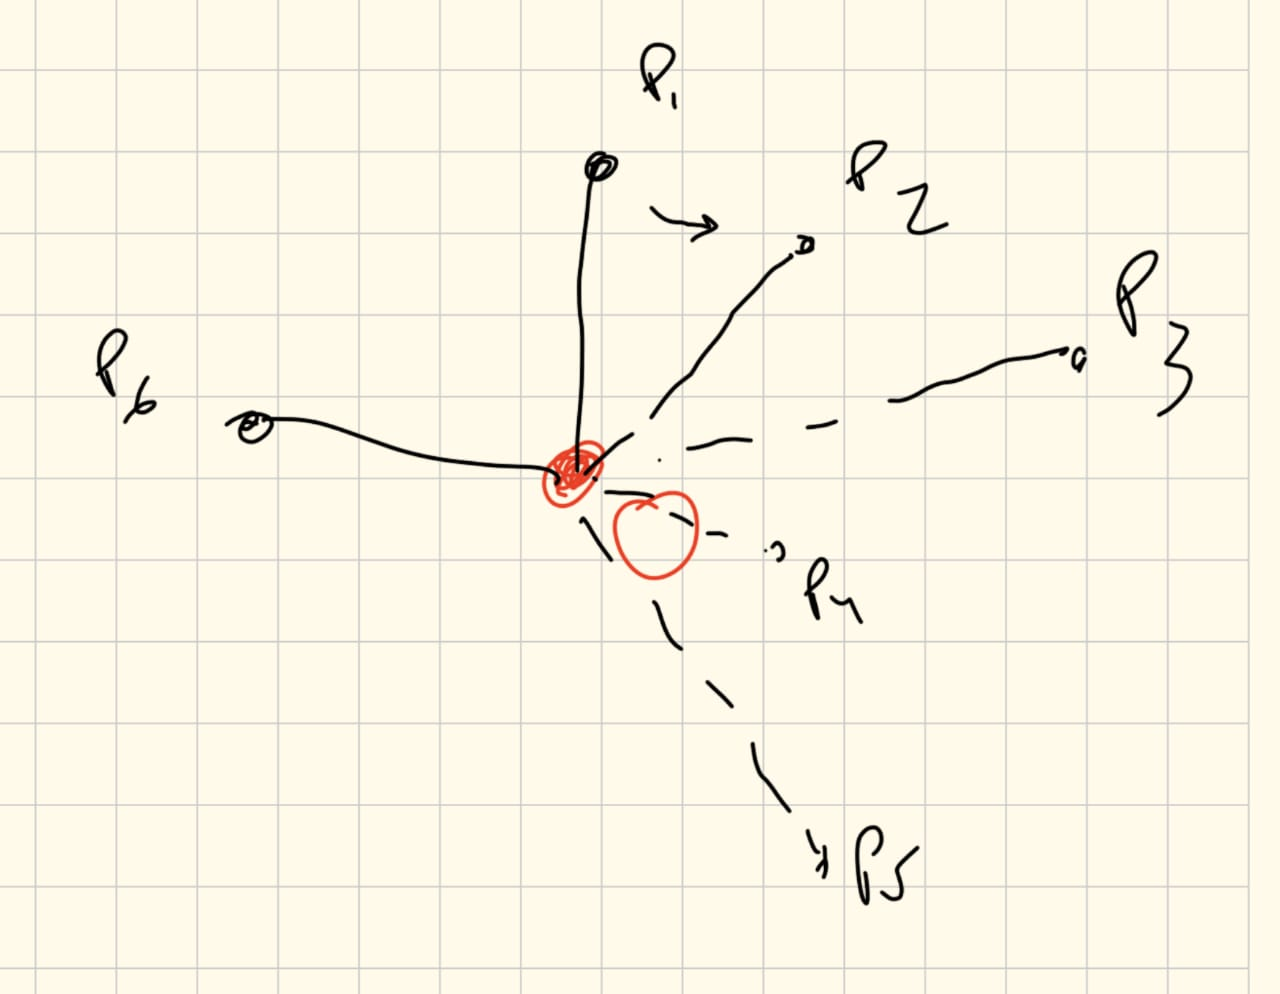
\includegraphics[scale=0.2]{Clockwise.jpeg}
\end{center}
Se dice ciclicamente porque cualquiera puede ser el primer punto, pero muchas veces se considera que inicia desde el rayo $+y$, en ese caso deja de ser ciclica y ahora es unica. 
\subsection{Componente Convexa}
\begin{definition}
    [Poligono convexo] Un poligono convexo es aquel que todas sus diagonales estan totalmente contenidas en el interior, cumplen que sus angulos interiores son siempre menores de $180^{\circ}$.
\end{definition}
\begin{definition}
    [Componente Convexa]
    Sea $S$ un conjunto finito de puntos. Entonces son todos colineales, o existe un unico subconjunto $P \in S$ de forma que los puntos en $P$ forman un poligono convexo y cada otro punto en $S$ esta adentro de ese poligono.  
\end{definition}
\begin{remark}
    Muchas veces se considera que si todos los puntos son colineales, su componente convexa es el segmento formado por los dos extremos.
\end{remark}

Una forma de ver que la componente convexa existe es tomar el punto con coordenada $x$ minima y que el siguiente punto de la componente convexa sea el primer punto del ordenamiento en sentido de las manecillas del reloj que inica en el rayo centrado en ese punto hacia $+y$. Para los siguientes puntos se inicia desde el rayo opuesto al segmento que se acaba de marcar. 
\begin{center}
    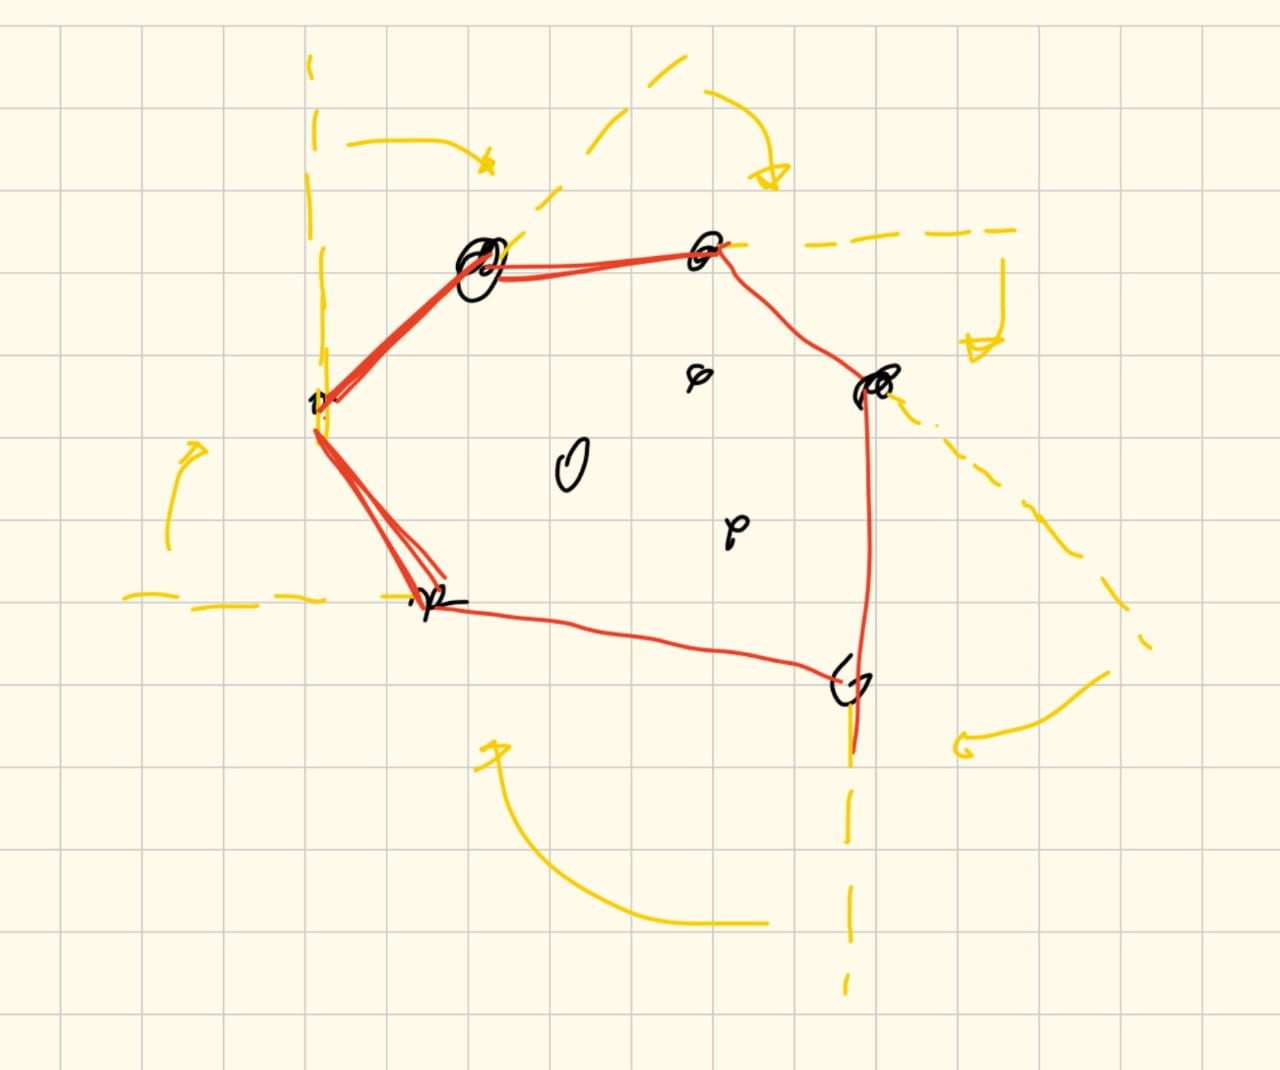
\includegraphics[scale=0.2]{ConvexHull.jpeg}
\end{center}

\begin{example}
    Prueba que para cualquiera 5 puntos, donde no hay 3 colineales, existen cuatro de ellos que forman un cuadrilatero convexo.
\end{example}

\begin{soln}
Vamos a hacer casos en base a cuantos vertices tiene su componente convexa. 
\begin{itemize}
    \item Si su componente convexa tiene 5 vertices, toma cualesquiera 4 de ellos y es un cuadrilatero convexo. 
    \item Si su componente convexa tiene 4 vertices, esos cuatro forman un cuadrilatero convexo.
    \item Si su componente convexa tiene 3 vertices, entonces hay 2 puntos en el interior. La recta que une esos dos puntos divide el plano en dos secciones, y en una por Casillas hay dos vertices de la componente convexa, considerando esos 2 más los dos puntos del interior obtienes un cuadrilatero convexo.
    \item No hay 3 colineales, entonces su componente convexa no puede tener $\leq 2$ vertices.
\end{itemize}
\end{soln}
\newpage
\section{Aproximadamente todos los problemas de geocombi de la historia (no)}
\epigraph{You'd have to stop the world just to stop the feeling}{"Good Luck, Babe!" - Chappell Roan }

\subsection{Nivel I}
\begin{problem}
 Sea $\Omega$ un conjunto de puntos en el plano, tal que cualquier punto en $\Omega$ es el punto medio del segmento formado por dos puntos de $\Omega$. Demuestra que $\Omega$ tiene infinitos puntos
\end{problem}

\begin{problem}
    Se tienen $n$ puntos en el plano. Cualquiera tres de ellos fomran un triangulo con area menor a $1$. Muestra que todos los puntos estan en un traingulo con un area menor o igual a $4$.
\end{problem}

\begin{problem}
Sea $S$ un conjunto de puntos en el plano en posición general. Prueba que los puntos $S$ pueden ser etiquetados $P_1,P_2, \ldots, P_k$ tal que la cadena $P_1P_2\ldots P_k$ no se interseca a si misma.
\end{problem}

\begin{problem}
    Se tiene un conjunto de puntos $ S $ en posición general, tal que para cada tres $A,B,C \in S$, el circuncentro de $\triangle ABC \in S$. Si $|S|\geq 3$, demuestra que $S$ es infinito.
\end{problem}

\begin{problem}
    Todos los puntos del plano son coloreados de rojo o de verde.Sea $A$ el conjunto de
todas las distancias que podemos encontrar entre dos puntos verdes y $B$ el conjunto
de todas las distancias que podemos encontrar entre dos puntos rojos. Muestra
que alguno de los conjuntos $A$ o $B$ contiene a todos los reales positivos.
\end{problem}

\begin{problem}
    En un cuadrado de $3\times 3$ se colocan 6 puntos. Muestra que dos de ellos estan a distancia menor que $2$.
\end{problem}

\begin{problem} % [Ibero 2024/4]
    We color some points in the plane with red, in such way that if $P,Q$ are red and $X$ is a point such that triangle $\triangle PQX$ has angles $30º, 60º, 90º$ in some order, then $X$ is also red. If we have vertices $A, B, C$ all red, prove that the barycenter of triangle $\triangle ABC$ is also red.
\end{problem}


\subsection{Nivel II}
\begin{problem} %[IMO 2015/1]
    We say that a finite set $\mathcal{S}$ of points in the plane is balanced if, for any two different points $A$ and $B$ in $\mathcal{S}$, there is a point $C$ in $\mathcal{S}$ such that $AC=BC$. We say that $\mathcal{S}$ is centre-free if for any three different points $A$, $B$ and $C$ in $\mathcal{S}$, there is no points $P$ in $\mathcal{S}$ such that $PA=PB=PC$.
\begin{itemize}
   
\item  Show that for all integers $n\ge 3$, there exists a balanced set consisting of $n$ points.

\item Determine all integers $n\ge 3$ for which there exists a balanced centre-free set consisting of $n$ points.
  
\end{itemize}
\end{problem}

\begin{problem}
    Find all integers $n \geq 2$ for which there exists a sequence of $2n$ pairwise distinct points $(P_1, \dots, P_n, Q_1, \dots, Q_n)$ in the plane satisfying the following four conditions:

\begin{itemize}
    \item no three of the $2n$ points are collinear;

\item $P_iP_{i+1} \ge 1$ for all $i = 1, 2, \dots ,n$, where $P_{n+1}=P_1$;
\item $Q_iQ_{i+1} \ge 1$ for all $i = 1, 2, \dots, n$, where $Q_{n+1} = Q_1$; and
\item $P_iQ_j \le 1$ for all $i = 1, 2, \dots, n$ and $j = 1, 2, \dots, n$.
\end{itemize}
\end{problem}

\begin{problem}
    En todo $n$-agono convexo existen tres vertices consecutivos $ABC$, tal que el circuncirculo de $ABC$ cubre todo el $n$-agono.
\end{problem}

\begin{problem} %[Balkan 2010/3]
    Una franja de ancho $w$ es el conjunto de todos los puntos que están sobre, o entre, dos rectas paralelas separadas por una distancia $w$. Sea $S$ un conjunto de $n$ puntos ($n \ge 3$) en el plano tal que cualesquiera tres puntos distintos de $S$ pueden ser cubiertos por una franja de ancho $1$.

Demuestra que $S$ puede ser cubierto por una franja de ancho $2$.
\end{problem}

\begin{problem} %[Sylverster-Gallay]
    Para todo conjunto finito de puntos en el plano $P$, se satisface alguna de las siguientes dos propiedades: Existe una recta $\ell$ que contiene a todos los puntos de $P$, o existe alguna recta $\ell$ que pasa por exactamente dos puntos de $P$.  
\end{problem}

\begin{problem} %[USA TSTST 2019/8]
    Let $\mathcal S$ be a set of $16$ points in the plane, no three collinear. Let $\chi(S)$ denote the number of ways to draw $8$ lines with endpoints in $\mathcal S$, such that no two drawn segments intersect, even at endpoints. Find the smallest possible value of $\chi(\mathcal S)$ across all such $\mathcal S$.
\end{problem}

\begin{problem} %[USAMO 2005/5]
    Let $n$ be an integer greater than 1. Suppose $2n$ points are given in the plane, no three of which are collinear. Suppose $n$ of the given $2n$ points are colored blue and the other $n$ colored red. A line in the plane is called a balancing line if it passes through one blue and one red point and, for each side of the line, the number of blue points on that side is equal to the number of red points on the same side.
Prove that there exist at least two balancing lines.
\end{problem}

\begin{problem} %[IMO 1989/3]
    Let $ n$ and $ k$ be positive integers and let $ S$ be a set of $ n$ points in the plane such that
\begin{itemize}
   
\item no three points of $ S$ are collinear, and

\item for every point $ P$ of $ S$ there are at least $ k$ points of $ S$ equidistant from $ P.$
 
\end{itemize}
Prove that:
\[ k < \frac {1}{2} + \sqrt {2 \cdot n}
\]
\end{problem}

\begin{problem} %[EGMO 2021/5]
    A plane has a special point $O$ called the origin. Let $P$ be a set of 2021 points in the plane such that
no three points in $P$ lie on a line and
no two points in $P$ lie on a line through the origin.
A triangle with vertices in $P$ is fat if $O$ is strictly inside the triangle. Find the maximum number of fat triangles.
\end{problem}

\begin{problem} %[IMSC 2025/4]
    Determine all $n$ such that it is possible to find a convex $n$-gon which can be tiled with triangles having angles $15^\circ$, $75^\circ$ and $90^\circ$.
\end{problem}

\begin{problem} %[Rioplantese 2012/3]
    	Let $T$ be a non-isosceles triangle and $n \ge 4$ an integer . Prove that you can divide $T$ in $n$ triangles and draw in each of them an inner bisector so that those $n$ bisectors are parallel.
\end{problem}

\begin{problem} %[IGO Intermedio 2022/4]
    We call two simple polygons $P, Q$ $\textit{compatible}$ if there exists a positive integer $k$ such that each of $P, Q$ can be partitioned into $k$ congruent polygons similar to the other one. Prove that for every two even integers $m, n \geq 4$, there are two compatible polygons with $m$ and $n$ sides. (A simple polygon is a polygon that does not intersect itself.)
\end{problem}

\subsection{Nivel III}
\begin{problem} %[IMO Shortlist 2019/C6]
    Let $n>1$ be an integer. Suppose we are given $2n$ points in the plane such that no three of them are collinear. The points are to be labelled $A_1, A_2, \dots , A_{2n}$ in some order. We then consider the $2n$ angles $$\angle A_1A_2A_3, \angle A_2A_3A_4, \dots , \angle A_{2n-2}A_{2n-1}A_{2n}, \angle A_{2n-1}A_{2n}A_1, \angle A_{2n}A_1A_2$$. We measure each angle in the way that gives the smallest positive value (i.e. between $0^{\circ}$ and $180^{\circ}$). Prove that there exists an ordering of the given points such that the resulting $2n$ angles can be separated into two groups with the sum of one group of angles equal to the sum of the other group.
\end{problem}

\begin{problem} %[IMO Shortlist 2000/G7]
    Ten gangsters are standing on a flat surface, and the distances between them are all distinct. At twelve o’clock, when the church bells start chiming, each of them fatally shoots the one among the other nine gangsters who is the nearest. At least how many gangsters will be killed?
\end{problem}

\begin{problem} %[IMO 2013/2]
    A configuration of $4027$ points in the plane is called Colombian if it consists of $2013$ red points and $2014$ blue points, and no three of the points of the configuration are collinear. By drawing some lines, the plane is divided into several regions. An arrangement of lines is good for a Colombian configuration if the following two conditions are satisfied:
\begin{itemize}
\item No line passes through any point of the configuration.

\item No region contains points of both colors.
\end{itemize}
Find the least value of $k$ such that for any Colombian configuration of $4027$ points, there is a good arrangement of $k$ lines.
\end{problem}

\begin{problem} %[RMM 2021/5]
    Let \(n\) be a positive integer. The kingdom of Zoomtopia is a convex polygon with integer sides, perimeter \(6n\), and \(60^\circ\) rotational symmetry (that is, there is a point \(O\) such that a \(60^\circ\) rotation about \(O\) maps the polygon to itself). In light of the pandemic, the government of Zoomtopia would like to relocate its \(3n^2+3n+1\) citizens at \(3n^2+3n+1\) points in the kingdom so that every two citizens have a distance of at least \(1\) for proper social distancing. Prove that this is possible. (The kingdom is assumed to contain its boundary.)
\end{problem}

\begin{problem} %[Ibero 2024/3]
    Let $O$ be a fixed point in the plane. We have $2024$ red points, $2024$ yellow points and $2024$ green points in the plane, where there isn't any three colinear points and all points are distinct from $O$. It is known that for any two colors, the convex hull of the points that are from any of those two colors contains $O$ (it maybe contain it in it's interior or in a side of it). We say that a red point, a yellow point and a green point make a bolivian triangle if said triangle contains $O$ in its interior or in one of its sides. Determine the greatest positive integer $k$ such that, no matter how such points are located, there is always at least $k$ bolivian triangles.
\end{problem}

\begin{problem} %[USA TSTST 2016/5]
    En el plano coordenado hay un número finito de muros, que son segmentos de recta disjuntos entre sí, ninguno de los cuales es paralelo a alguno de los ejes. Un bulldozer comienza en un punto arbitrario y se mueve en la dirección $+x$. Cada vez que golpea un muro, gira en un ángulo recto con respecto a su trayectoria, alejándose del muro, y continúa moviéndose. (Por lo tanto, el bulldozer siempre se mueve paralelo a los ejes).

Demuestra que es imposible que el bulldozer golpee ambos lados de cada muro.
\end{problem}

\begin{problem} %[IOI 2006]
    Varios puntos azules y rojos se colocan en un cuadrado con las siguientes propiedades:
    \begin{itemize}
        \item Las dos esquinas superiores son puntos rojos.
        \item Las dos esquinas inferiores son azules.
        \item No hay tres puntos colineales.
    \end{itemize}
    Prueba que es posible dibujar sementos rojos entre puntos rojos y segmentos azules entre puntos azules de manera que todos los puntos rojos est\'an conectados, y todos los puntos azules est\'an conectados.
    \begin{center}
        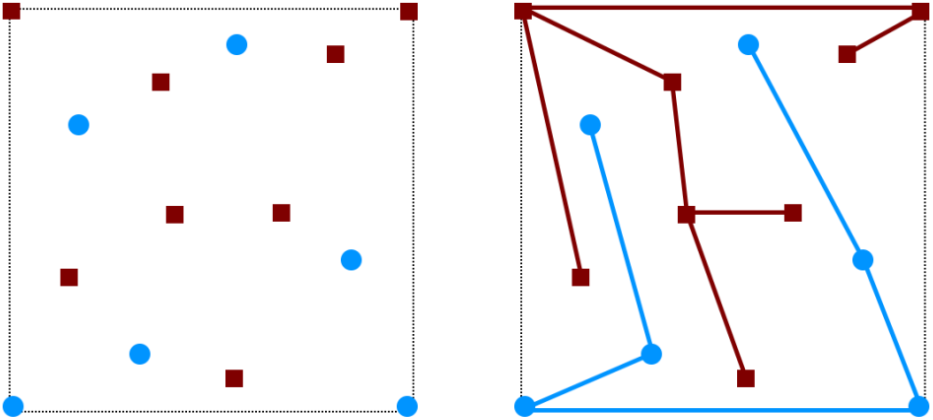
\includegraphics[scale = 0.23]{IOI 2005.png}
    \end{center}
\end{problem}

\begin{problem} %[IMO Shortlist 2008/G5]
    Let $ k$ and $ n$ be integers with $ 0\le k\le n - 2$. Consider a set $ L$ of $ n$ lines in the plane such that no two of them are parallel and no three have a common point. Denote by $ I$ the set of intersections of lines in $ L$. Let $ O$ be a point in the plane not lying on any line of $ L$. A point $ X\in I$ is colored red if the open line segment $ OX$ intersects at most $ k$ lines in $ L$. Prove that $ I$ contains at least $ \dfrac{1}{2}(k + 1)(k + 2)$ red points.
\end{problem}

\begin{problem} %[China TST 2022/16]
    Find all positive integer $k$ such that one can find a number of triangles in the Cartesian plane, the centroid of each triangle is a lattice point, the union of these triangles is a square of side length $k$ (the sides of the square are not necessarily parallel to the axis, the vertices of the square are not necessarily lattice points), and the intersection of any two triangles is an empty-set, a common point or a common edge.
\end{problem}

\begin{problem} %[China TST 2011/13]
    	Given positive integer $ n \ge 5 $ and a convex polygon $P$, namely $ A_1A_2...A_n $. No diagonals of $P$ are concurrent. Proof that it is possible to choose a point inside every quadrilateral $ A_iA_jA_kA_l (1\le i<j<k<l\le n) $ not on diagonals of $P$, such that the $ \tbinom{n}{4} $ points chosen are distinct, and any segment connecting these points intersect with some diagonal of $P$.
\end{problem}

\begin{problem} %[Ibero 2013/6]
    A beautiful configuration of points is a set of $n$ colored points, such that if a triangle with vertices in the set has an angle of at least $120$ degrees, then exactly 2 of its vertices are colored with the same color. Determine the maximum possible value of $n$.
\end{problem}

\subsection{Nivel IV}

\begin{problem} %[IMO 2014/6]
    A set of lines in the plane is in general position if no two are parallel and no three pass through the same point. A set of lines in general position cuts the plane into regions, some of which have finite area; we call these its finite regions. Prove that for all sufficiently large $n$, in any set of $n$ lines in general position it is possible to colour at least $\sqrt{n}$ lines blue in such a way that none of its finite regions has a completely blue boundary.
\end{problem}

\begin{problem} %[RMM 2018/5 Leak]
    	Two ants are moving along the edges of a convex polyhedron. The route of every ant ends in its starting point, so that one ant does not pass through the same point twice along its way. On every face $F$ of the polyhedron are written the number of edges of $F$ belonging to the route of the first ant and the number of edges of $F$ belonging to the route of the second ant. Is there a polyhedron and a pair of routes described as above, such that only one face contains a pair of distinct numbers?
\end{problem}

\begin{problem} %[IMO 2011/2]
    Let $\mathcal{S}$ be a finite set of at least two points in the plane. Assume that no three points of $\mathcal S$ are collinear. A windmill is a process that starts with a line $\ell$ going through a single point $P \in \mathcal S$. The line rotates clockwise about the pivot $P$ until the first time that the line meets some other point belonging to $\mathcal S$. This point, $Q$, takes over as the new pivot, and the line now rotates clockwise about $Q$, until it next meets a point of $\mathcal S$. This process continues indefinitely.
Show that we can choose a point $P$ in $\mathcal S$ and a line $\ell$ going through $P$ such that the resulting windmill uses each point of $\mathcal S$ as a pivot infinitely many times.
\end{problem}

\begin{problem} %[China TST 2011/2]
    Let $S$ be a set of $n$ points in the plane such that no four points are collinear. Let $\{d_1,d_2,\cdots ,d_k\}$ be the set of distances between pairs of distinct points in $S$, and let $m_i$ be the multiplicity of $d_i$, i.e. the number of unordered pairs $\{P,Q\}\subseteq S$ with $|PQ|=d_i$. Prove that $\sum_{i=1}^k m_i^2\leq n^3-n^2$.
\end{problem}

\begin{problem} %[RMM 2011/5]
    	For every $n\geq 3$, determine all the configurations of $n$ distinct points $X_1,X_2,\ldots,X_n$ in the plane, with the property that for any pair of distinct points $X_i$, $X_j$ there exists a permutation $\sigma$ of the integers $\{1,\ldots,n\}$, such that $\textrm{d}(X_i,X_k) = \textrm{d}(X_j,X_{\sigma(k)})$ for all $1\leq k \leq n$.
(We write $\textrm{d}(X,Y)$ to denote the distance between points $X$ and $Y$.)
\end{problem}

\begin{problem} %[RMM 2015/6]
    Given a positive integer $n$, determine the largest real number $\mu$ satisfying the following condition: for every set $C$ of $4n$ points in the interior of the unit square $U$, there exists a rectangle $T$ contained in $U$ such that

$\bullet$ the sides of $T$ are parallel to the sides of $U$;

$\bullet$ the interior of $T$ contains exactly one point of $C$;

$\bullet$ the area of $T$ is at least $\mu$.
\end{problem}

\begin{problem} %[IMO 2020/6]
    Prove that there exists a positive constant $c$ such that the following statement is true:
Consider an integer $n > 1$, and a set $\mathcal S$ of $n$ points in the plane such that the distance between any two different points in $\mathcal S$ is at least 1. It follows that there is a line $\ell$ separating $\mathcal S$ such that the distance from any point of $\mathcal S$ to $\ell$ is at least $cn^{-1/3}$.

(A line $\ell$ separates a set of points S if some segment joining two points in $\mathcal S$ crosses $\ell$.)

Note. Weaker results with $cn^{-1/3}$ replaced by $cn^{-\alpha}$ may be awarded points depending on the value of the constant $\alpha > 1/3$.
\end{problem}

\end{document}